\documentclass{article} % For LaTeX2e
\usepackage{nips14submit_e,times}
\usepackage{hyperref}
\usepackage{url}
\usepackage{amsmath}
\usepackage{amssymb}
\usepackage{algorithm}
\usepackage[noend]{algpseudocode}
\usepackage{graphicx}
\usepackage[labelfont=bf]{caption}
%\documentstyle[nips14submit_09,times,art10]{article} % For LaTeX 2.09

\DeclareMathOperator{\rvec}{rvec}

\title{A Tractable Model for High-Dimensional Real Valued Sequences}


\author{
David S.~Hippocampus\thanks{ Use footnote for providing further information
about author (webpage, alternative address)---\emph{not} for acknowledging
funding agencies.} \\
Department of Computer Science\\
Cranberry-Lemon University\\
Pittsburgh, PA 15213 \\
\texttt{hippo@cs.cranberry-lemon.edu} \\
\And
Coauthor \\
Affiliation \\
Address \\
\texttt{email} \\
\AND
Coauthor \\
Affiliation \\
Address \\
\texttt{email} \\
\And
Coauthor \\
Affiliation \\
Address \\
\texttt{email} \\
\And
Coauthor \\
Affiliation \\
Address \\
\texttt{email} \\
(if needed)\\
}

% The \author macro works with any number of authors. There are two commands
% used to separate the names and addresses of multiple authors: \And and \AND.
%
% Using \And between authors leaves it to \LaTeX{} to determine where to break
% the lines. Using \AND forces a linebreak at that point. So, if \LaTeX{}
% puts 3 of 4 authors names on the first line, and the last on the second
% line, try using \AND instead of \And before the third author name.

\newcommand{\fix}{\marginpar{FIX}}
\newcommand{\new}{\marginpar{NEW}}

%\nipsfinalcopy % Uncomment for camera-ready version

\begin{document}


\maketitle

\begin{abstract}
We present a probabilistic model for generating and modelling high dimensional real-valued sequences. This model combines a powerful distribution estimator, the Real-Valued Neural Autoregressive Density Estimator (RNADE) with a Recurrent Neural Network (RNN) for capturing temporal dependencies in sequences of high dimensional data. Maximum likelihood learning can be applied to efficiently train the model using a gradient based optimiser. Unlike other models in this family, log-likelihoods for sequences can be computed exactly and efficiently. We evaluate the model's performance on standard datasets and compare its performance to other models. 
\end{abstract}

\section{Introduction}
\label{intro}
Modeling sequences is a fundamental problem in machine learning. Speech, music, video and many other kinds of naturally occurring data are sequential in nature. A good sequential model can be used for discriminative tasks, for sequence completion, as a prior in more complex tasks, sequence denoising and various other applications. There are many existing models such as Linear Dynamical Systems and Hidden Markov Models (HMMs) that model sequential data. Although these models are used extensively in many fields such as speech, audio and music, they can only model a limited a history. Modelling long term dependencies between data points becomes intractable when using these models \cite{sutskever2007learning}. 
%Although HMMs are widely used in speech recognition and a wide variety of other problems, they are limited by the exact form of their latent representation and become computationally infeasible for modelling long histories \cite{sutskever2007learning}. 

Recurrent Neural Networks (RNNs) are simple and powerful models for sequential data. RNNs have an internal memory that allows them to model dependencies between observations separated by a variable number of time steps. In principle RNNs can describe relationships between inputs separated by arbitrary lengths of time. However in practice, training RNNs using gradient based optimisers is not easy and their use in practical applications has been limited. After being ignored by machine learning researchers for a long time, there has been a resurgence of interest in RNNs over the last decade. There have been several key developments in understanding and solving some of the issues associated with gradient based training of RNNs \cite{Martens2011,bengio2012advances}. These advances have made it possible to train RNNs on various tasks and RNNs have been shown to be very successful on a variety of music and language applications \cite{mikolov2011empirical,Boulanger-Lewandowski2012,bengio2012advances}. 

An RNN can either be used to map an input sequence to an output sequence or it can be used as a generative model. Generative models try to model the entire space of inputs given a finite number of training examples. In its simplest form, the RNN can predict unimodal outputs under the assumption that all the output variables are conditionally independent given the remaining outputs. However for many problems this is not satisfactory. A more powerful RNN-based generative model can be constructed by letting the RNN predict the parameters of a powerful distribution estimator. Employing this architecture we obtain complex high-dimensional distributions at each time-step conditioned on the previous inputs. This idea was first employed in the Recurrent Temporal Restricted Boltzmann Machine (RTRBM) \cite{Sutskever2008} model. The model was then extended by combining an RNN with a Neural Autoregressive Distribution Estimator (NADE) and the RBM via a more general architecture \cite{Boulanger-Lewandowski2012}. The RNN-RBM and the RNN-NADE have been successfully used for tasks in speech and music \cite{boulangerphone,Boulanger-Lewandowski2012}. 

Although the models described above have been successful on various tasks, they are unsuitable for modelling real-valued data. Both the RBM and the NADE are designed to explicitly model binary vectors. If the input data lies in $[0,1]$, then the RBM can be used via the mean-field approximation. Unbounded data can be modelled by using gaussian visible units and bernoulli hidden units. However these extensions of the RBM to real data have several known limitations \cite{theis2011all}. In this paper, we present a new model for real-valued sequential data by combining the RNN with the RNADE. The RNADE is a density estimator that has been shown to outperform gaussian mixture models (GMMs) and a host of other density estimators on several tasks \cite{Uria2013}. We show that obtaining probabilities and log-likelihoods from the combined RNN-RNADE model is tractable and fast. We show that the gradients with respect to the model parameters can be calculated exactly and that training can be easily performed with a gradient based optimiser. We evaluate the model's performance on real-valued datasets and demonstrate a marked improvement in performance. 

%Modeling sequences is a fundamental problem in machine learning. Many popular models like Hidden Markov Models (HMMs) and Linear Dynamical Systems use latent variables to capture temporal properties of sequential model. However HMMs employ a 1-of-K state representation for the hidden state and trying to model larger histories can lead to exponentially large hidden states. RNNs are an interesting alternative for modeling sequential data and have recently been employed in speech recognition, MIR and various other tasks. RNNs employ a deterministic distributed hidden representation that can in theory capture temporal properties over very long time scales. However RNNs are limited by the effectiveness of gradient based optimisers and the size of the output space that they can model. To rectify this issue, a family of models that condition complex distribution estimators on the hidden state of an RNN have been proposed. The first such model was the RTRBM and it was later extended by the RNN-RBM and the RNN-NADE \cite{Boulanger-Lewandowski2012,}. 

%The main idea behind this family of models is to use complex distribution estimators like the RBM and the NADE and incorporate a temporal element by conditioning the parameters of the model at each time step on previously observed parts of the sequence. As mentioned before an RNN can in theory learn dependencies over large time-scales within the data and is used in these models for conditioning the distributions at each step. RNN based models are also attractive because the recurrent parts of the model can be easily trained by using BPTT or Hessian Free (HF) optimisation. The RTRBM and the RNN-NADE models cannot be trained exactly by maximum likelihood learning because the gradients of the RBMs cannot be computed exactly. This problem was rectified by using a NADE instead of an RBM. However, this family of temporal models is not very well suited to modeling real-valued data. Both the RBM and the NADE estimate distributions over binary spaces. Although the RBM can be used on real data by either scaling the data between $[0,1]$ or by using the Gaussian-Bernouilli RBM (gRBM), we feel that using an estimator meant for real data could provide further gains. 

%In this paper, we propose a model called the RNN-RNADE that combines the temporal modeling properties of the RNN with the recently proposed RNADE model. The RNADE is a generalisation of the NADE to real-valued data. It has been shown to outperform gaussian mixture models (GMMS) and many other distribution estimators on a variety of datasets of varying dimensionality and complexity. In this paper we explore how the RNADE can be combined with the RNN to yield a temporal generative model. We show how the model can be trained efficient using maximum likelihood learning using gradient based optimisers. Finally we evaluate the performance  

%Recently various neural based models have been proposed for learning modelling high dimensional sequential data. These models have been shown to work much better than standard models such as HMMs and Linear Dynamical Systems. These models include the TRBM, the RTRBM and the RNN-RBM. Although these models work very well for complex high dimensional data, they have several limitations. They cannot be trained exactly because their gradients can't be computed. Also obtaining probabilities from the model is not tractable and often very expensive. These models also suffer from the fact, that the distribution estimators they use are meant for binary data. Even though these models can be extended to model real-value with some approximations, these models are known to have several short-comings. The RNN-NADE is a tractable alternative, however it is unsatisfactory, because the NADE can only model distributions over high-dimensional binary vectors. In this paper we propose a tractable distribution estimator for high-dimensional real-valued sequences by making use of the RNADE which was proposed recently. The proposed model can be trained and sampled from efficiently by back-propagating error gradients through the computational graph. A key advantage of this model over other neural-based sequence models is that getting the likelihoods of the occurrence of sequences is tractable and fast. Because of this, the model can be easily combined with other sequence models and is applicable to various tasks like sequence completion, sequence denoising and classification of complex real-valued sequences. We compare our model's performance to the earlier models and demonstrate its many benefits. 
 
\section{Recurrent Neural Networks as generative models}
\label{RNN}
%An RNN can define a distribution over sequences $\mathbf{x}_1^{T}$ if the loss function is of the form $ L = \sum_{t} -\log p(\mathbf{x}^{t+1};\boldsymbol{\theta}^{t})$ where $p(.;\boldsymbol{\theta})$ is a distribution with parameters $\boldsymbol{\theta}$, and $\boldsymbol{\theta}^t \equiv f(\mathbf{x}_1^t)$. In more detail, according to figure 1, let the hidden state of the RNN at time $t$ be give by:
%$$ \mathbf{h}_{RNN}^t = \sigma(\mathbf{W}_{in}\mathbf{x}^t + \mathbf{W}_{rec}\mathbf{h}_{RNN}^{t-1} + \mathbf{b}_{RNN})$$
%Let the hidden state of the RNN at time $t-1$ be used to output $\mathbf{z}^{t} = \sigma(\mathbf{W}_{out}\mathbf{h}_{RNN}^{t-1} + \mathbf{b}_{out})$ and let the parameters of the distribution at time $t$, $\boldsymbol{\theta}^t = f(\mathbf{z}^t,\boldsymbol{\theta}_{model})$ where $\boldsymbol{\theta}_{model}$ are the independent parameters of the distribution estimator and $f$ is some differentiable function with respect to the model parameters. If we can obtain the derivates of the cost function with respect to the parameters of the distribution $p(;|\boldsymbol{\theta})$, then it can be shown that the parameters of the RNN can be trained by using the chain rule and Back Propagation Through Time (BPTT). Therefore:

% $$ \frac {\partial L}{\partial{\theta^t}} = -\frac {\partial p(\mathbf{x}^t)}{\partial \theta^t}$$
% $$ \frac {\partial L}{\partial{\theta_{model}}} = \sum_{t} -\frac {\partial p(\mathbf{x}^t)}{\partial{\theta_{model}}}   $$

% $$ \frac {\partial L}{\partial{\mathbf{z}^t}} = \sum_{T} \sum_{i} -\frac {\partial p(\mathbf{x}^t)}{\partial{\theta^i}} \frac {\partial f(\mathbf{z}^t,\boldsymbol{\theta}_{model})^i}{\partial{\mathbf{z}^t}}  $$

% Once we obtain all the errors with respect to the outputs of the RNN, the gradients with respect to the RNN parameters can be easily found by applying the chain rule further and backpropagating the gradients back in time. We show the calculations for the proposed model in section 3. Further derivations of the results can be found in the supplementary material. 

% The RTRBM \cite{Sutskever2008} was the first model that uses the above idea to condition RBMs on the outputs of an RNN. However, the model is constrained by the fact that the outputs of RNN are responsible for both the density estimation and for propagating temporal information to the following time step. The RNN-RBM \cite{Boulanger-Lewandowski2012} generalises the RTRBM model by introducing a separate hidden layer for the RNN. Decoupling the states of the RNN and conditional RBMs led to an improvement in performance. 

% The RNN-RBM model cannot be trained exactly because the error derivatives with respect to the parameters of the conditional RBMs are approximated using Contrastive Divergence (CD). Another drawback of the RNN-RBM model is that obtaining the log-likelihood of the sequence is intractable. This is because the RBM defines a joint distribution over the observed and hidden variables. Obtaining probabilities over the observed variables implies a summation over an exponential number of hidden states. These shortcomings can be addressed by replacing the RBM with the NADE, which is a tractable distribution estimator with performance comparable to RBMs. The log-likelihood can be easily calculated and more powerful gradient based optimisers like HF \cite{Martens2011} can be applied because the gradients are exactly calculable. 

\begin{figure}
	\centering
    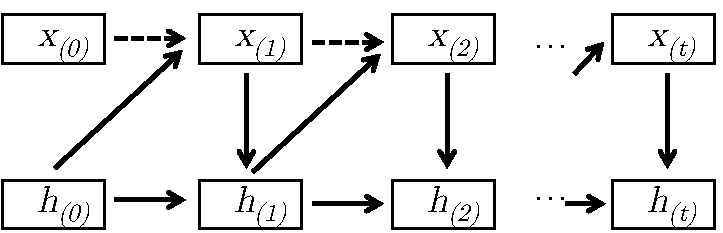
\includegraphics[scale=0.8]{RNN.pdf}
    \caption{Graphical structure of the generative RNN. Broken arrows indicate optional connections for temporal smoothing.}
    \label{fig:rnade}
\end{figure}


An RNN defines a distribution over an output sequence $ \mathbf{x} \equiv \left\{ \mathbf{x}^t \in \mathbb{R}^n, t \leq T \right\}$ in the following manner:
$$ P(\mathbf{x}) = \prod_{t=1}^{T} P(\mathbf{x}^t|\mathcal{A}^t)$$
where $\mathcal{A}^t \equiv \left\{ \mathbf{x}^{\tau}|\tau < t \right\}$ is the history of the input sequence $\mathbf{x}$ until time $t$, $P(\mathbf{x}^t|\mathcal{A}^t)$ is the probability of observing $\mathbf{x}^t$ conditioned on the history of the sequence $\mathcal{A}^t$. RNN based generative models with different properties and capacities can be constructed by carefully choosing the form and parameterization of the conditional $P(\mathbf{x}^t|\mathcal{A}^t)$ as discussed later in this section. 

In an RNN with a single hidden layer, the hidden state at time $t$ is given by:
\begin{equation}
\label{rnn-hidden}
\mathbf{h}^t = \sigma{(W_{in}\mathbf{x}^t + W_{rec}\mathbf{h}^{t-1} + \mathbf{b}_h)}
\end{equation}
where $W_{in}$ is the weight matrix from the input to the hidden layer, $W_{rec}$ is the recurrent weight matrix from the previous hidden state to the current state and $\mathbf{b}_h$ is the bias vector for the hidden layer. In a standard RNN, the next time step $\mathbf{x}^{t+1}$ is predicted as:
$$ \mathbf{x}^{t+1} = \sigma{(W_{out}\mathbf{h}^{t} + \mathbf{b}_{out})}$$  
where $W_{out}$ connects the hidden layer to the output layer and $\mathbf{b}_{out}$ is the output bias. As shown in Figure \ref{fig:rnn}, there can be optional connections between the input and the input from the previous time-step for temporal smoothing. However as mentioned earlier, each of the outputs is unimodal and independent of the other outputs. 
These assumptions are too restrictive for many real-world problems and have given rise to a new family of RNN-based generative models with high-dimensional multi-modal conditional distributions at each time-step. Such a model can be realised by letting the hidden layer of the RNN predict parameters of a distribution estimator just like in a mixture density network \cite{bishop1994mixture}.  

In previous work \cite{Boulanger-Lewandowski2012}, the RNN was used to predict the hidden and visible biases of an RBM and a NADE model to yield complex conditional distributions at each time step. Although these models are very good at modelling sequences of binary vectors, they are unsuitable for modelling real-valued data. It is easy to show that any distribution estimator can be used provided the gradients of the cost function with respect to the parameters of the density estimator are obtainable. The combined model can then be trained by maximising the likelihood of the training set and using back-propagation through time (BPTT) \cite{rumelhart1985learning}. In order to use the power of this architecture for modelling real data, we present a model that combines the RNN and the RNADE. The RNADE is discussed in detail in the following section and the combined model is described in Section \ref{RNN-RNADE}. 

\section{The RNADE}
\label{RNADE}

\begin{figure}
	\centering
    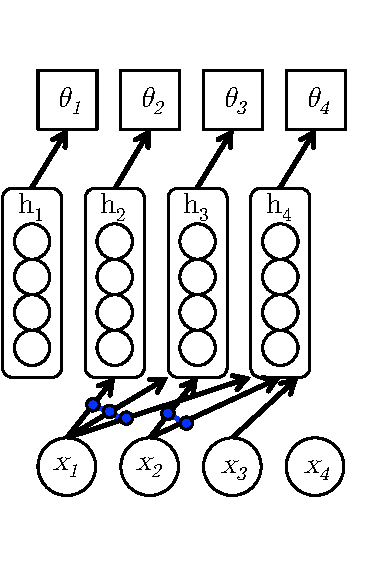
\includegraphics[scale=0.7]{RNADE.pdf}
    \caption{Graphical structure of the RNADE. The blue dots indicate that the weights coming out from a node are tied. $\theta_{d}$ denote the parameters of the mixture density network for the dimension $d$. }
    \label{fig:rnn-rnade}
\end{figure}


The RNADE is a generalisation of the NADE to model real-valued data. Like the NADE, the RNADE expresses the joint probability of the data as a product of one-dimensional conditional distributions as follows:
$$ p(x) = \prod_{d=1}^{D} p(x_d|\mathbf{x_{<d}}) \: \text{with} \: p(x_d|\mathbf{x_{<d}}) = p_{\mathcal{M}(x_d|\theta_d)} $$ where $p_{\mathcal{M}}$ is a mixture of Gaussians and $\boldsymbol{x}_{<d}$ is a vector of all the dimensions of the data point $<d$. The RNADE is computationally efficient because of the weight sharing employed in the calculation of the hidden state: %The hidden state The RNADE models each of the conditional distributions by means of a feed-forward neural network with tied weights, with one neural network for each dimension. The activations of the hidden units are calculated as follows:

$$ \mathbf{a}_d = \boldsymbol{W}_{.,<d}\boldsymbol{x}_d + \mathbf{c}$$
$$ \boldsymbol{h}_d = \sigma (\rho_d \mathbf{a}_d)$$


where $\mathbf{c} \in \mathbb{R}^{H}$ and $\boldsymbol{W} \in \mathbb{R}^{D \times (H-1)}$ are neural network parameters that are shared across all the neural networks and $\sigma(x) = 1/(1+e^{-x})$ is the sigmoid function. $\boldsymbol{W}_{.,<d}$ represents the first $d-1$ columns of the shared weight matrix. The term $\rho_d$ is a scaling factor which is also learnt from the data. The scaling factor was introduced in \cite{AISTATS2011_Bengio11} in order to prevent the sigmoid hidden units from saturating. The computation of the activations of the hidden units can be made more efficient by performing the computation as:
$$ \mathbf{a}_1 = \mathbf{c}, \: \: \; \mathbf{a}_{d+1} = \mathbf{a}_{d} + x_d \mathbf{W}_{.,d}$$

 Unlike the NADE which models each output as a bernouilli distribution, the outputs of each of the feed forward neural networks of the RNADE are mixtures of Gaussians. Therefore the RNADE comprises of $D$ mixture density networks with tied input-to-hidden weights. Once the hidden units of the RNADE have been computed, they are used to compute the parameters of the GMMs $\boldsymbol{\theta}_d  = \left\{ \boldsymbol{\alpha}_d, \boldsymbol{\mu}_d, \boldsymbol{\sigma}_d \right\}$ at each output, where $\boldsymbol{\alpha}_d$ are the mixing coefficients, $\boldsymbol{\mu}_d$ are the means and $\boldsymbol{\sigma}_d$ are the variances. These parameters are computed as follows:

$$ \boldsymbol{\alpha}_d = \text{softmax} ({\mathbf{V}_{d}^{\alpha}}^T \mathbf{h}_d + \mathbf{b}^{\alpha}_{d})$$
$$ \boldsymbol{\mu}_d = {\mathbf{V}_{d}^{\mu}}^T \mathbf{h}_d + \mathbf{b}^{\mu}_{d}$$
$$ \boldsymbol{\sigma}_d = \exp ({\mathbf{V}_{d}^{\sigma}}^T \mathbf{h}_d + \mathbf{b}^{\sigma}_{d})$$

where $ \mathbf{V}_{d}^{\alpha},\mathbf{V}_{d}^{\mu},\mathbf{V}_{d}^{\sigma}$ are $H \times K$ matrices , $\mathbf{b}^{\alpha}_{d},\mathbf{b}^{\mu}_{d},\mathbf{b}^{\sigma}_{d}$ are vectors of size $K$ and $K$ is the number of components in the GMM. More concisely, the RNADE is parameterised by $\mathbf{V}^{\alpha},\mathbf{V}^{\mu},\mathbf{V}^{\sigma}$ which are $D \times H \times K$ matrices and $\mathbf{b}^{\alpha},\mathbf{b}^{\mu},\mathbf{b}^{\sigma}$ which are matrices of size $D \times K $.
The parameters of the RNADE can be learnt by performing gradient ascent on the log-likelihood given a training set. 

\section{RNN-RNADE}
\label{RNN-RNADE}

\begin{figure}
	\centering
    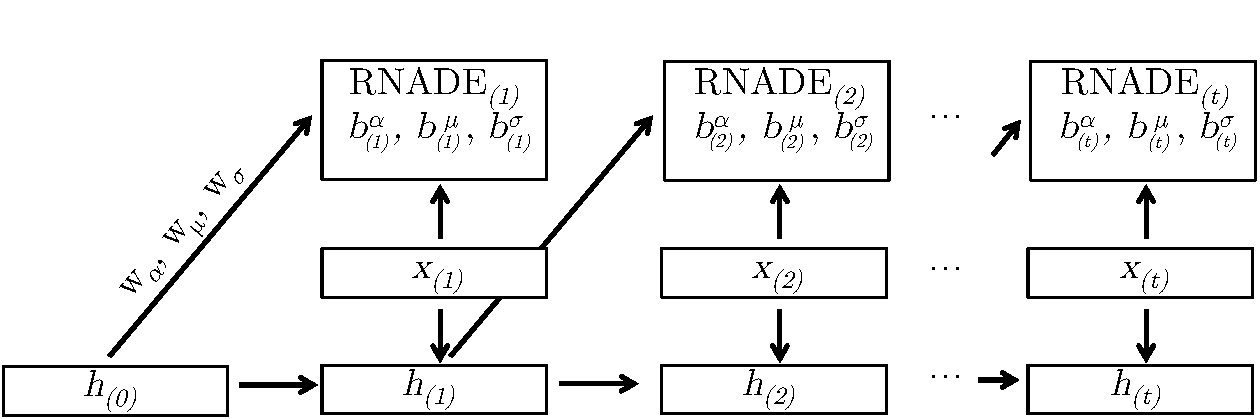
\includegraphics[scale=0.65]{RNN-RNADE.pdf}
    \caption{Graphical structure of the RNN-RNADE. The hidden state of the RNN at time $t$ predicts the parameters of the RNADE at $t+1$. }
    \label{fig:rnn-rnade}
\end{figure}


The RNN-RNADE is a sequence of conditional distributions for each time-step of a sequence $\mathbf{x}$. As shown in Figure \ref{fig:rnn-rnade}, the parameters of the conditional distributions at each time step $t$ are a function of the hidden state of the RNN at the previous time-step $t-1$. We first define the notation in order to simplify discussion of the training algorithm later in the section. 

From section \ref{RNADE}, the RNADE is parameterised by $ \theta \equiv \left\{ \mathbf{V}^{\alpha},\mathbf{V}^{\mu},\mathbf{V}^{\sigma},\mathbf{b}^{\alpha},\mathbf{b}^{\mu},\mathbf{b}^{\sigma} \right\}$. Let  $ \theta_t \equiv \left\{ \mathbf{V}^{\alpha}_{t},\mathbf{V}^{\mu}_{t},\mathbf{V}^{\sigma}_{t},\mathbf{b}^{\alpha}_{t},\mathbf{b}^{\mu}_{t},\mathbf{b}^{\sigma}_{t} \right\}$ denote the parameters of the conditional RNADE at time $t$. Although all the parameters of the RNADE at time $t$ can be a function of the hidden state at $t-1$, we consider the matrices $ \mathbf{V}^{\alpha},\mathbf{V}^{\mu},\mathbf{V}^{\sigma}$ to be fixed at each time step and only consider the biases $\mathbf{b}^{\alpha},\mathbf{b}^{\mu},\mathbf{b}^{\sigma}$ to be time-dependent through the RNN hidden state. This constraint significantly reduces the number of parameters that need to be estimated and makes the model and training computationally more efficient. 
Therefore, $ \theta_t \equiv \left\{ \mathbf{V}^{\alpha},\mathbf{V}^{\mu},\mathbf{V}^{\sigma},\mathbf{b}^{\alpha}_{t},\mathbf{b}^{\mu}_{t},\mathbf{b}^{\sigma}_{t} \right\}$. As described later, we experiment with the architecture to ascertain which permutation of time dependent parameters $\mathbf{b}^{\alpha}_{t},\mathbf{b}^{\mu}_{t},\mathbf{b}^{\sigma}_{t}$ gives the best results.  

The time-dependent RNADE parameters are give by:
\begin{equation}
\label{one}
\rvec(\mathbf{b}^{\alpha}_{t}) = \rvec(\mathbf{b}^{\alpha}) + W_{\alpha}\mathbf{h}^{t-1}
\end{equation}
\begin{equation}
\label{two}
\rvec(\mathbf{b}^{\mu}_{t}) = \rvec(\mathbf{b}^{\mu}) + W_{\mu}\mathbf{h}^{t-1}
\end{equation}
\begin{equation}
\label{three}
\rvec(\mathbf{b}^{\sigma}_{t}) = \rvec(\mathbf{b}^{\sigma}) + W_{\sigma}\mathbf{h}^{t-1}
\end{equation}
where $\rvec(A) = [a_{1,1}, ..., a_{1,n}, a_{2,1}, ..., a_{2,n}, ..., a_{m,1}, ..., a_{m,n}]$ for some $m \times n$ matrix $A$, $W_{\alpha},W_{\mu},W_{\sigma} \in \mathbb{R}^{r \times D c}$ are matrices from the hidden state of the RNN to the mixing coefficients, means and standard deviations of the RNADE respectively, $r$ is the number of hidden units in the RNN, $D$ is the dimensionality of the input vectors and $c$ is the number of components of each GMM in the RNADE. 

%Therefore using equations \ref{one},\ref{two},\ref{three} we can obtain the time-dependent biases for the RNADE at each time step. 

\subsection{Learning in the RNN-RNADE}

The model can be trained by minimising the negative log-likelihood of training sequences using gradient descent. The cost function is given by:
\begin{align}
L(\theta) &= - \log P(\mathbf{x}) \nonumber\\ 
&= -\sum_{t=1}^{T} \log P(\mathbf{x}^t;\theta^t) \label{cost}
\end{align}

The gradients of the conditionals $P(\mathbf{x}^t;\theta^t)$ with respect to the parameters of the RNADE can be calculated, the details of which are outlined in \cite{Uria2013}. Once we obtain the gradients with respect to the time-dependent parameters, the entire network can be trained using BPTT. 

From Equation \ref{cost}, $\frac{\partial L}{\partial \mathbf{b}^{\alpha}_{t}} = \frac{\partial (-P(\mathbf{x}^t;\theta^t))}{\partial \mathbf{b}^{\alpha}_{t}}$ which can be easily obtained as shown in \cite{Uria2013}. The derivatives of the cost with respect to the other time-dependent parameters can be obtained in a similar manner. Once we obtain $ \frac{\partial L}{\partial \mathbf{b}^{\alpha}_{t}}, \frac{\partial L}{\partial \mathbf{b}^{\mu}_{t}}, \frac{\partial L}{\partial \mathbf{b}^{\sigma}_{t}}$, the gradients with respect to the other model parameters can be calculated as follows:

\begin{equation}
\frac{\partial L}{\partial W_{\alpha}} = \sum_{t=1}^T \frac{\partial L}{\partial \mathbf{b}^{\alpha}_{t}} {\mathbf{h}^{t-1}}^{T}
\end{equation}
\begin{equation}
\frac{\partial L}{\partial W_{\mu}} = \sum_{t=1}^T \frac{\partial L}{\partial \mathbf{b}^{\mu}_{t}} {\mathbf{h}^{t-1}}^{T}
\end{equation}
\begin{equation}
\frac{\partial L}{\partial W_{\sigma}} = \sum_{t=1}^T \frac{\partial L}{\partial \mathbf{b}^{\sigma}_{t}} {\mathbf{h}^{t-1}}^{T}
\end{equation}

Using equations \ref{rnn-hidden},\ref{one},\ref{two},\ref{three}:

\begin{equation}
\label{grad-hidden}
\frac{\partial L}{\partial \mathbf{h}^t} = W_{rec}\frac{\partial L}{\partial \mathbf{h}^{t+1}} \mathbf{h}^{t+1} (1 - \mathbf{h}^{t+1}) + W_{\alpha} \frac{\partial L}{\partial \mathbf{b}^{\alpha}_{t+1}} + W_{\mu} \frac{\partial L}{\partial \mathbf{b}^{\mu}_{t+1}} + W_{\sigma} \frac{\partial L}{\partial \mathbf{b}^{\sigma}_{t+1}}
\end{equation}

Using equation \ref{grad-hidden}, the gradients with respect to the remaining model parameters can be calculated easily. 

$$ \frac{\partial L}{\partial \mathbf{b}_{h}} =  \sum_{t=1}^{T} \frac{\partial L}{\partial \mathbf{h}^t} \mathbf{h}^t (1 - \mathbf{h}^t)$$
$$ \frac{\partial L}{\partial W_{rec}} = \sum_{t=1}^{T} \frac{\partial L}{\partial \mathbf{h}^t} \mathbf{h}^t (1 - \mathbf{h}^t) {\mathbf{h}^{t-1}}^T$$
$$ \frac{\partial L}{\partial W_{in}} = \sum_{t=1}^{T} \frac{\partial L}{\partial \mathbf{h}^t} \mathbf{h}^t (1 - \mathbf{h}^t) {\mathbf{x}^{t}}^T$$

As shown above, the gradients of the cost function with respect to the model parameters can be obtained with BPTT and used to train the joint model. In our implementation of the model, we used the automatic differentiation library Theano \cite{bergstra+al:2010-scipy} instead of calculating the gradients by hand. In the supplementary material, we provide further details about the exact form of the gradients. Unlike the RNN-RBM, the gradients of the RNN-RNADE model can be calculated exactly. Therefore model training can benefit from the use of more powerful gradient based optimiser like the Hessian Free optimiser \cite{Martens2011}

\section{Experiments}
\label{Experiments}
The RNN-RNADE is tested on three tasks, a simple 2-D trajectory, videos of bouncing balls and motion capture data. On all three tasks we report the squared prediction error, allowing comparisons between our approach and the RTRBM and RNN-RBM in the latter two tasks. Code for experiments is available in the supplementary material.  A grid search was carried out on the hyperparameters, including the number of hidden neurons in the RNADE, the number of recurrent hidden neurons, the number of components and the learning rate. Experiments were run for 100,000 updates, where the model is trained on a single randomly chosen sequence. Early stopping was employed, comparing the model's score on a validation set. Additionally, training was halted if the log likelihood became positive.

%In all experiments, the RNADE was fixed to use 1 component per input dimension.

\subsection{2-D stochastic trajectory}
This task is used as a demonstrative example of the system. At each time step a particle's 2-D coordinates are determined by the system of equations:

\(x = N(\sin(t)+1,0.1)\)\\
\(y = x N(\sin(t+0.5)+1,0.2)\)

where $t$ is the timestep. The model is trained on sequences of 100 consecutive timesteps. The model comprised of 20 hidden units for both the RNN and the RNADE. The squared prediction error per frame is $\mathbf{0.16}$. The motivation behind performing this task was to devise a toy problem for quickly evaluating the effects of changes made to the model or the training algorithm. Although the task is quite simple and could be solved by simpler sequential models, visually inspecting predictions helped us verify the effectiveness of the learning algorithm and isolate certain issues with training that are discussed in detail later in this section. Videos showing the predictions made by the model are available in the supplementary material. 

\subsection{Motion capture data}
As in \cite{Sutskever2008} and \cite{Boulanger-Lewandowski2012} we use the human motion capture dataset which represents sequences of joint angles, translations and rotations of the base of the spine. The data consists 49 real-valued dimensions at each time-step and is therefore ideal for evaluating the performance of the proposed model. As mentioned earlier, we performed a grid search on some of the hyper-parameters. The model that performed the best comprised of $100$ hidden units for the RNADE and $200$ hidden units for the RNN. The best squared prediction error was $\mathbf{7.26\%}$ which is a significant improvement over the over the RTRBM ($20.1\%$) and the RNN-RBM ($16.2\%$). 

\subsection{Videos of bouncing balls}
The bouncing balls dataset consists of synthetic videos of three balls bouncing in a box, as described in \cite{Sutskever2008}. We used videos of 15x15 pixels (225 dimensions) of 3 balls bouncing and sequences of 128 frames. Each pixel is a real value in the range $[0,1]$. The RNADE is not ideal for this problem since the input space is bounded but the GMMs at the RNADE outputs model the entire space. In our experiments the best model comprised of $300$ hidden units for the RNN and $200$ hidden units for the RNADE. The best squared prediction error we achieved was $2.04$ which is of the same order as the RTRBM ($2.11$) but much worse compared to the RNN-RBM ($0.96$). In order to get a better understanding of the problem we inspected the samples produced by the conditional distributions. We observed that in a large proportion of frames there were a few samples which were very noisy i.e. their values were much greater than 1 or much less than 0. These samples contributed to higher squared prediction errors. Clipping the samples drawn from the RNADE at $0$ and $1$ did not have any significant effect on the squared prediction error. We generated sequences of bouncing balls from the model similar to \cite{Sutskever2008}, however the noisy samples (even with clipping) when used as inputs degrade the future samples quickly and we did not obtain smooth sequences. 
%As the RNADE samples from a Gaussian distribution, it is possible for illegal values to be produced and so the output of the model is constrained to the minimum and maximum values of the data. Using an RNADE with 1 component per dimension and 200 hidden neurons per dimension and 200 recurrent neurons in the RNN, the RNN-RNADE achieves a squared test error per frame of 2.1, similar to the RTRBM but substantially higher than the RNN-RBM as reported in \cite{Boulanger-Lewandowski2012}. Videos of errors per frame can be found in the supplementary material.

\section{Discussion}
\label{Discussion}
In this section we provide details and discuss the important aspects of the training procedure.
\subsection{Gradient Descent}
 The training algorithm was set to perform 100000 updates, where one sequence was used to compute the gradients for the update. In our experiments we found that the model reached lower validation errors when momentum was used during gradient descent. We used a constant momentum rate of $0.9$ in all our experiments. We found that using high learning rates would either the cause the gradients to blow up quickly or force the parameters to saturate at local minimas within a small number of epochs. We found a learning rate of $0.001$ to be ideal and linearly decreasing the learning every epoch seemed to help training. 

The problem of exploding or vanishing gradients is a well documented problem while training RNNs and was one of the primary reasons that research on RNNs was abandoned for a long time. In our initial experiments on the mocap dataset we found that the gradients would explode even when using extremely small learning rates. The problem of exploding gradients is probably more acute for the RNN-RNADE because of the highly non-linear relationship between the parameters of the RNN and the RNADE and the negative log-likelihood cost function. We used gradient clipping \cite{bengio2012advances} to deal with this issue. Gradient clipping uses a simple heuristic to deal with the problem of exploding gradients. If the norm of the gradient $g$ for some update is above a threshold, then the gradient is rescaled to $(\frac{\tau}{\left\lVert g \right\rVert})g$, where $\tau$ is the threshold. In our experiments we set the threshold to 50, which was the average of the norm of the gradients of 1000 randomly generated sequences. 

\subsection{Overfitting}
 Although the training algorithm was set up to perform a large number of updates, on all three problems we noticed that the negative log-likelihood cost approaches zero very quickly. For example on the mocap dataset, the cost approaches zero after 2000 updates. Once the cost becomes negative, it can continue to reach arbitrarily low values without having much effect on the validation error. This demonstrates that the RNN-RNADE is prone to overfitting to the training data. The RNN-RNADE is more susceptible to this phenomenon than the RNADE of mixture density networks because the mean for a data point at $t$ is a function of the hidden state of the RNN at $t-1$. As the model is trained, the predictions from the RNN become more accurate and after a point the means come very close to the data points causing the log-likelihood to become positive. It is not obvious how this problem can be dealt with since the means are functions of the hidden state of the RNN and the RNN gets better at predicting the means as training continues. We tried a few obvious strategies such as penalising the weights from the RNN to the RNADE to prevent them from becoming too large but this did not seem to affect the problem of overfitting. Having observed this, we used the training cost as a stopping criterion and stopped training when log-likelihood becomes positive. However even with this issue, the model seems to learn very quickly (within 2000 updates on the mocap dataset) and still outperform the RNN-RBM by a relative improvement of $> 50\%$. 

\subsection{Architecture}

As mentioned earlier, we only allow the bias parameters of the RNADE $\mathbf{b}^{\alpha},\mathbf{b}^{\mu},\mathbf{b}^{\sigma}$ be time dependent. It is not obvious which combination of time dependent biases would yield the optimal model. In our experiments with the mocap and bouncing balls dataset, we trained models with all possible combinations of time-dependent biases, with the obvious exception of the case where none of the biases are time-dependent. We observed that a time dependent $\mathbf{b}^{\mu}$ was crucial for the model to capture temporal dependencies. Whenever $\mathbf{b}^{\mu}$ was omitted from the set of time-dependent parameters, the model failed to learn. We found that time-dependent $\mathbf{b}^{\mu},\mathbf{b}^{\sigma}$ yielded the best models. Making $\mathbf{b}^{\alpha}$ time dependent did not lead to better training, in fact a time dependent $\mathbf{b}^{\alpha}$ exacerbates the issue of overfitting during training. 

Another parameter that was crucial in determining test performance was the number of components in the GMM at the RNADE outputs. GMMs when trained with a large number of components are known to cause overfitting \cite{bishop2006pattern}. We found that if we set the number of components to be greater than 2, then the model overfit very quickly during training and these models could not generalise to test data. Best results were obtained when the number of components was limited to $2$ components, with not much difference in performance between GMMs with $1$ or $2$ components.  

\section{Conclusions and Future Work}

In this paper we introduced the RNN-RNADE which is a powerful probabilistic model for real-valued high dimensional sequences. We evaluated its performance and obtained a significant improvement in performance over previously proposed models from the same family. The model can be easily trained with gradient descent and probabilities are easy to obtain unlike other models. However there are some issues with the model that need to be investigated further. In the future we would like to study the issue of overfitting. The model could potentially perform much better if overfitting was reduced. We would also like to study the effect of more powerful gradient based optimisers like Hessian Free on model training. 

\label{conclusion}

\bibliography{bibliography}
\bibliographystyle{plain}
\end{document}
